% This must be in the first 5 lines to tell arXiv to use pdfLaTeX, which is strongly recommended.
\pdfoutput=1
% In particular, the hyperref package requires pdfLaTeX in order to break URLs across lines.
\pdfminorversion=7
\pdfobjcompresslevel=3
\pdfcompresslevel=9


\documentclass[11pt]{article}

% Change "review" to "final" to generate the final (sometimes called camera-ready) version.
\usepackage{acl}

% pour gérer les figures et tableaux avec H
\usepackage{float}
% tableaux plus propres
\usepackage{booktabs}

% Standard package includes
\usepackage{times}
\usepackage{latexsym}

% For proper rendering and hyphenation of words containing Latin characters (including in bib files)
\usepackage[T1]{fontenc}

% This assumes your files are encoded as UTF8
\usepackage[utf8]{inputenc}

\usepackage{amsmath}

% This is not strictly necessary, and may be commented out,
% but it will improve the layout of the manuscript,
% and will typically save some space.
\usepackage{microtype}

% This is also not strictly necessary, and may be commented out.
% However, it will improve the aesthetics of text in
% the typewriter font.
\usepackage{inconsolata}

%Including images in your LaTeX document requires adding
%additional package(s)
\usepackage{graphicx}

\title{Défi DEFT 2009 : Classifier automatiquement les groupes politiques}

\author{
  \text{MANSERI Kéhina\textsuperscript{(1)(2)}}
  \text{SIRVEN-VIENOT Alix\textsuperscript{(1)(2)}}
  \text{VAN-DEN-ZANDE Débora\textsuperscript{(1)(3)}}
\\
\\
  \textsuperscript{(1)}Université Paris Nanterre
  \textsuperscript{(2)}Parcours Recherche et Développement
  \textsuperscript{(3)}Parcours Pro
\\
\\
    \small {
    manserikehina@gmail.com, alix.vienot@gmail.com, vdzdebora@gmail.com
    }
\\
}

\begin{document}
\maketitle
\begin{abstract}
La classification des interventions parlementaires en fonction de leur parti politique représente une tâche clé dans la fouille de textes. Dans le cadre du défi DEFT 2009, nous avons analysé un corpus multilingue comprenant des interventions en français, anglais et italien. Ce corpus présente des défis liés au déséquilibre des classes et à la diversité des thématiques. Pour relever ce défi, nous avons testé plusieurs algorithmes de classification. 

EN ANGLAIS AUSSI ???


\end{abstract}

\section{Introduction}
Notre objectif est d'entraîner un modèle qui détermine automatiquement le parti politique d’appartenance de chaque intervenant dans le corpus parlementaire. 
Vous pouvez retrouver notre travail sur notre GitHub\footnote{\url{https://github.com/KehinaleK/deft09/tree/main}} pour accéder à l'entièreté de notre code.

\section{Présentation des données}
Notre corpus est multilingue, c'est-à-dire qu'il contient plusieurs ensembles dans des langues différentes telles que le français, l'anglais et l'italien. C'est donc un corpus parallèle et comparable auquel nous avons affaire. 

\subsection{Extraction des données}
Nous avons extrait les données sur le site du DEFT\footnote{\url{https://deft.lisn.upsaclay.fr/}} en format xml et nous les avons parsé avec BeautifulSoup. 

En comparant la longueur de la liste de labels et les ID des échantillons de test, nous avons pu remarquer que deux interventions ne disposaient pas de label. Nous avons donc décidé de simplement les ignorer.


\subsection{Suppression des doublons}
Après concertation avec les autres étudiants, nous avons été informées qu'il y avait des doublons entre les ensembles de train et de test.

Nous avons trouvé au total 7 813 textes en communs entre les données d'entraînement et de test. Nous voulions donc retirer ces doublons des deux ensembles tout en essayant de respecter le répartition du corpus qui est de base de 60\% des échantillons pour le train et 40\% pour le test. 

En effet, retirer tous les doublons de l'ensemble de train nous donnerait un split bien trop proche.

Après avoir enlevé les doublons, nous avons obtenu un split de 53,40\% pour le train et 46,60\% pour le test. Pour avoir une distribution exacte de 60/40, nous avons retiré certains textes de l'ensemble de test.

\subsection{Distribution des classes}
Voici à quoi ressemblent nos classes une fois la suppression des données et l'égalisation du split (cf. Tableau~\ref{tab:pourcentage_test}).

\begin{table}[ht]
\centering
    \begin{tabular}{lccc}
        \toprule
        \textbf{Classe}   & \textbf{Train} & \textbf{Test} & \textbf{Pourcentage} \\ \midrule
        \textbf{PSE}      & 3650           & 2489          & 40.54\% \\    
        \textbf{ELDR}     & 1351           & 908           & 40.19\% \\          
        \textbf{Verts-ALE}& 1609           & 1072          & 39.99\% \\          
        \textbf{PPE-DE}   & 4635           & 3047          & 39.66\% \\          
        \textbf{GUE-NGL}  & 1823           & 1196          & 39.62\%  \\ \bottomrule            
    \end{tabular}
    \caption{Distribution des pourcentages entre Train et Test.}
    \label{tab:pourcentage_test} % Tableau~\ref{tab:pourcentage_test}
\end{table}

\textbf{Résumé des totaux} \\
Total Train : \> 13068 \\
Total Test  : \> 8712 \\
Pourcentage Global Test : \> 40.00\%
\\

À première vue, les classes semblent déséquilibrées. Afin de mieux visualiser cette disparité, nous avons réalisé un graphique. La distribution des classes dans les différents splits est présentée sur la Figure~\ref{fig:graph_avant}.

\begin{figure}[H]
  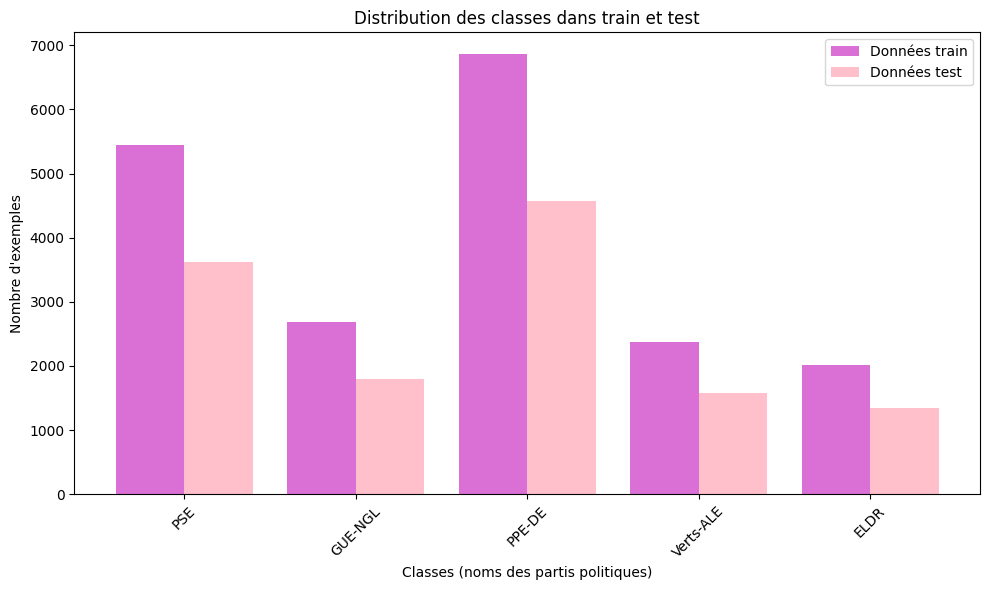
\includegraphics[width=\columnwidth]{latex/graphique_avant.png}
  \caption{Répartition des classes \textbf{avant} nettoyage et rééquilibrage du split}
  \label{fig:graph_avant} % pareil pour citer Figure~\ref{fig:graph_avant}
\end{figure}



\begin{figure}[H]
  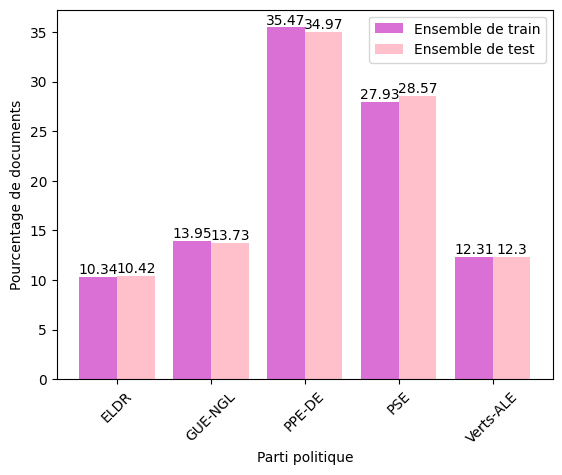
\includegraphics[width=\columnwidth]{latex/graphique_apres.png}
  \caption{Répartition des classes \textbf{après} nettoyage et rééquilibrage du split}
  \label{fig:graph_apres} % Figure~\ref{fig:graph_apres}
\end{figure}


\section{Pré-traitement des données}
\subsection{Normalisation des données}
Pour préparer nos textes à la classification, nous avons appliqué plusieurs étapes de normalisation. Les ponctuations et les \textit{stopwords} ont été supprimés pour réduire le bruit dans les données. Tous les textes ont été convertis en minuscules pour uniformiser leur format. Enfin, une lemmatisation a été effectuée pour ramener les mots à leur forme canonique, optimisant ainsi la qualité et la cohérence des données textuelles.

\subsection{Vectorisation des données}
Dans l'article présent sur le site \cite{forest2009variation}, on voit que les paramètres de la vectorisation jouent un rôle assez important dans les performances d'une modèle.

En nous basant sur cet article et sur le TP1, nous allons tester le TFIDF Vectorizer avec différents hyperparamètres sur trois classifieurs différents afin de voir si nous obtenons des résultats significativement mieux. Les classifieurs utilisés seront : KNN (car utilisé dans l'article) SVC Lineaire (modèle linéaire) Complement NB (modèle probabilistique)

Si pour tous ces algorithmes, une vectorisation donne de meilleurs résultats, alors nous utiliserons cette dernières pour le reste de nos tests.

Au vu de nos résultats, on peut admettre que c'est un tfidf avec une max df de 0.9, des max\_features de 15 000 et un ngram range de (1, 2) qui donne les meilleurs résultats. Nous utiliserons ainsi cette combinaison d'hyperparamètres et donc cette vectorisation pour nos essais suivants.

\section{Comparaison des modèles}
Nous avons décidé de tester plusieurs modèles qui ont des types de classifications différentes (cf. Tableau~\ref{tab:classifieurs_types}).

\begin{table}[h]
    \centering
    \begin{tabular}{|l|l|}
        \hline
        \textbf{Nom du Classifieur}        & \textbf{Type} \\ \hline
        LinearSVC                         & Linéaire      \\ \hline
        RandomForestClassifier            & Ensemble      \\ \hline
        KNeighborsClassifier              & Non-linéaire  \\ \hline
        PassiveAggressiveClassifier       & Linéaire      \\ \hline
        MultinomialNB                     & Probabiliste  \\ \hline
        ComplementNB                      & Probabiliste  \\ \hline
        SVC                               & Non-linéaire  \\ \hline
        RidgeClassifier                   & Linéaire      \\ \hline
        LGBMClassifier                    & Ensemble      \\ \hline
        LogisticRegression                & Linéaire      \\ \hline
        SGDClassifier                     & Linéaire      \\ \hline
    \end{tabular}
    \caption{Liste des classifieurs et leur type.}
    \label{tab:classifieurs_types} % ça c'est pour le citer après ! Tableau~\ref{tab:classifieurs_types}
\end{table}

\subsection{Choix des algorithmes}
Dans cette étude, nous avons essayé plusieurs modèles, incluant des approches linéaires, probabilistes, non-linéaires et d'ensemble, dans le but de comparer leurs performances et d'analyser l'impact du déséquilibre des classes. Les modèles linéaires, généralement moins efficaces dans ce contexte, ont été comparés à des modèles probabilistes (MultinomialNB, ComplementNB) et d'ensemble (Random Forest, LGBMClassifier), connus pour leur aptitude à mieux gérer les données déséquilibrées.

À l'issue de nos tests, nous avons retenu les trois meilleurs algorithmes, [ALGOS]

\subsection{Organisation de la comparaison}

\section{Stratégies d'amélioriation}
Pour améliorer nos résultats, on pourrait essayer de faire un downsampling ou un upsampling, c'est-à-dire d'augmenter ou de diminuer le nombre d'échantillons dans nos données. Avoir des données équilibrées est une chose importante dans le machine learning car sinon les algorithmes priviligent les classes majoritaires et les résultats sont donc médiocres.

Dans notre cas, comme on a pas énormément de données, le plus intéressant serait d'augmenter artificiellement nos données. Heuresement, sklearn propose de le faire assez facilement grâce au module resample.

Pour le upsampling, on augmente les données minoritaires au même nombre d'échantillons que la classe qui en a le plus, et pour le downsampling, on fait la même chose mais avec la classe minimale. Les résultats sont disponibles sur la Figure~\ref{fig:equilibrage}.

\begin{figure}[H]
  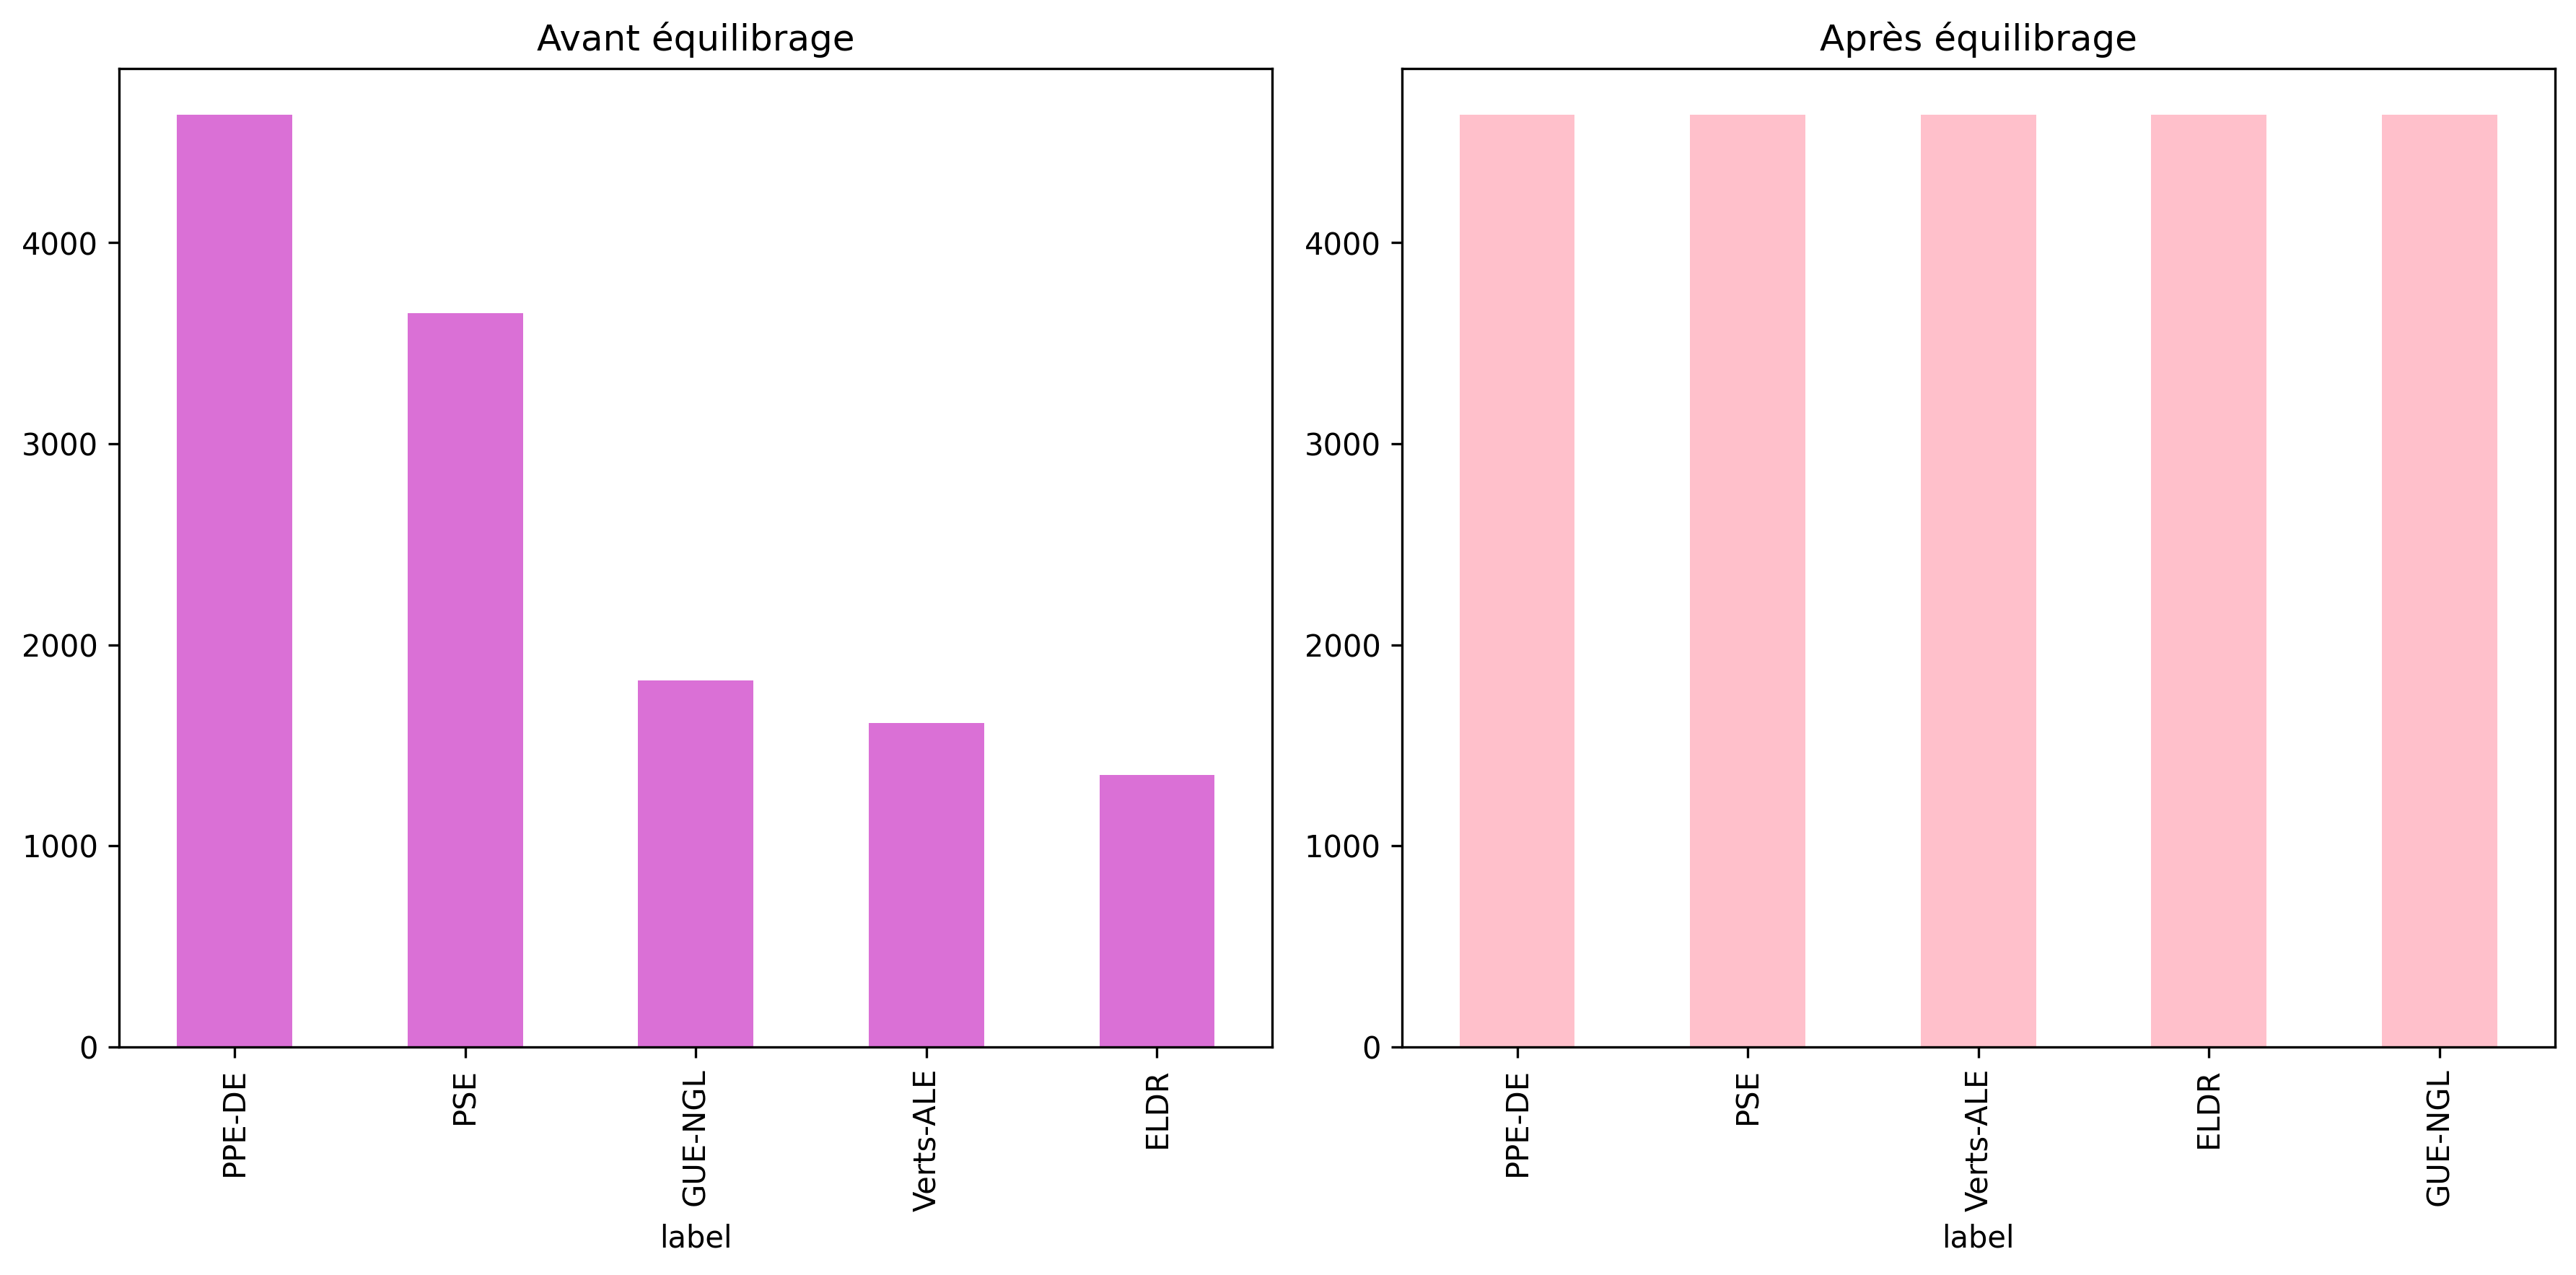
\includegraphics[width=\columnwidth]{latex/equilibrage.png}
  \caption{Répartition des classes \textbf{avant} nettoyage et rééquilibrage du split}
  \label{fig:equilibrage} % pareil pour citer Figure~\ref{fig:equilibrage}
\end{figure}

\section{Évaluation des modèles}

\subsection{Métriques d'évaluation}
\begin{table}[ht]
    \centering
    \begin{tabular}{lccc}
        \toprule
        \textbf{Algorithme} & \textbf{Précision} & \textbf{Rappel} & \textbf{F1-score} \\ \midrule
        Logistic Regression & 0.85               & 0.82            & 0.83              \\
        Random Forest       & 0.88               & 0.85            & 0.86              \\
        SVM                 & 0.87               & 0.84            & 0.85              \\ \bottomrule
    \end{tabular}
    \caption{Résultats des algorithmes sur les métriques de classification.}
    \label{tab:resultats_algo}
\end{table}

\subsection{Analyse des résultats}


\section{Conclusion}


\bibliography{custom}
\cite{forest2009variation}

\end{document}